\documentclass[12pt,a4paper]{article}
\usepackage{lastpage}
\usepackage{fancyhdr}
\pagestyle{fancy}
\usepackage{ dsfont }
\usepackage{hyperref}
\usepackage{graphicx}
\usepackage{subcaption}
\usepackage{float}
\usepackage{multirow}
\usepackage{array}
\usepackage{geometry}
\geometry{
    left=2cm,
    right=2cm,
    top=2cm,
    bottom=2cm
}
\usepackage{setspace}
\onehalfspacing
\usepackage{listings}
\bibliographystyle{IEEEtran}
\usepackage{xcolor}
\lstset{
    language=C++,                  % Set your language (you can change it as needed)
    basicstyle=\ttfamily\small,     % The basic style of your code
    keywordstyle=\color{blue},      % Keyword style
    stringstyle=\color{red},        % String literal style
    commentstyle=\color{gray},     % Comment style
    morecomment=[l][\color{magenta}]{\#},  % Directive style (like #include)
    numbers=left,                   % Line numbers on left
    numberstyle=\tiny\color{gray},  % Line number style
    stepnumber=1,                   % Line number step
    numbersep=5pt,                  % How far the line numbers are from the code
    backgroundcolor=\color{white},  % Background color for code block
    tabsize=2,                      % Tab size
    showspaces=false,               % Show spaces adding particular underscores
    showstringspaces=false,         % Underline spaces within strings only
    showtabs=false,                 % Show tabs within strings adding particular underscores
    frame=single,                   % Adds a frame around the code
    captionpos=b,                   % Sets the caption-position to bottom
    breaklines=true,                % Sets automatic line breaking
    breakatwhitespace=false,        % Sets if automatic breaks should only happen at whitespace
    escapeinside={\%*}{*)},         % If you want to add LaTeX within your code
}

\rhead{2131917, Page~\thepage~of~\pageref{LastPage}}
\newcolumntype{M}[1]{>{\centering\arraybackslash}p{#1}}
\begin{document}
\begin{center}
    \section*{HumanMade: A Platform for Verified Human Creations}
    \textbf{Author:} Luca Sarif-Kattan\\
    \textbf{Supervisor:} Ligang He\\
    \textbf{Year of study:} 2024\\
    \textbf{Keywords:} AI, Generative AI, Human, Creations, Blockchain, Web App, Node.js, Neural Network
\end{center}

\newpage

\noindent \textbf{Abstract:} With the dawn of generative AI, the landscape of human creativity and ingenuity is increasingly encroached upon. It is clear to most experts that this trend will continue in some fashion \cite{aiimpacts}, and there is a high chance that the entire creative space will be heavily dominated by AI in the near future. Due to the anthropocentric worldviews many of us hold \cite{anthropocentric} and to retain the pride of the human identity, having a platform which supports and incentivises human creation seems like it will be an in-demand product, and a beneficial necessity. HumanMade seeks to do this whilst avoiding the flawed approach of directly detecting AI-generated content, by:
\begin{itemize}
    \item Giving humans an easy way to document and upload their Creations
    \item Ensuring Creations are tamper-proof and traceable to the original creator
    \item Enabling and empowering the community of users to decide what they think is human-made and deserves their attention
\end{itemize}

\vspace{10pt}
\noindent \textbf{Acknowledgements:} I would like to thank myself for my amazing ideas, skilled programming and genius-level problem solving. I would like to thank Ligang He for a frictionless and enjoyable supervisor experience.

\newpage
\tableofcontents
\newpage

\section{Motivators}
\subsection{The Generative AI Explosion}
We are currently (March of 2024) in the midst of a generative AI (GAI) arms race. ChatGPT managed to reach 100 million users in 2 months \cite{gptstatistics}. Incredible advancements are being made weekly. More broadly, experts are predicting High-Level Machine Intelligence by 2059 \cite{aiimpacts}, and this is an exponentially decaying timeline, down 8 years from the previous time the survey was given. Here are some of the main reasons for this current AI explosion:
\begin{itemize}
    \item \textbf{Advancements in hardware.} The architectures which a lot of these models are based off of were discovered a while ago, (for example, the seminal Attention Is All You Need paper was released in 2017 \cite{attention}), but recently we have witnessed huge improvements in the AI accelerated hardware needed to scale these models. Examples include Google's development of the TPU \cite{tpu}, and Nvidia's development of the Ampere architecture line of GPUs. GAI models require large-scale compute for the training phase. 
    \begin{figure}[H]
        \centering
        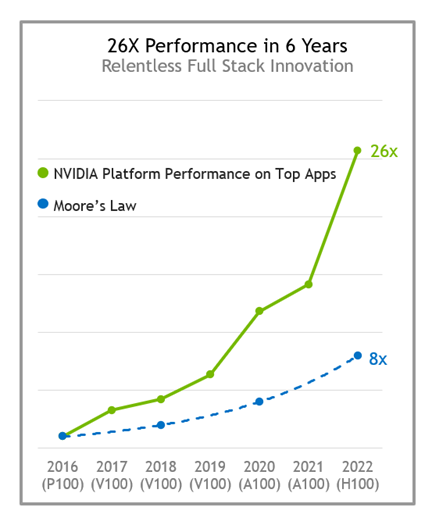
\includegraphics[scale=0.6]{nvidiaGraph.png}
        \cite{nvidia}
        \caption{A comparison of Nvidia hardware progress compared to Moore's law. The A100 GPU was used to train OpenAI's GPT-4. \cite{gpt4}}
    \end{figure}

    \item \textbf{Lack of regulations and restrictions.} There are currently no restrictions on the development of such technologies in the US, and the EU has introduced limited restrictions in the new AI act \cite{aiact}. There are obvious geopolitical incentives to allow the acceleration of GAI technologies, and open letters calling to pause giant AI experiments have failed to bring action \cite{fol}.
    \item \textbf{Profit incentives.} Such technologies are applicable across a huge spectrum of high-level tasks. There was 14 billion dollars in funding in 2023 towards GAI technologies \cite{genfunding}.
\end{itemize}
\subsection{A Look at the SOTA}
 A big part of the motivation for such a project comes from the unbelievable progress and ability of current GAI models, and how we might attempt to improve their detection. Therefore, in this section we take a brief look into the current state-of-the-art in GAI. At the moment there are two dominant model types:
\begin{itemize}
    \item Transformer models, used for text generation
    \item Diffusion models, used for image and video generation
\end{itemize}
Transformers were initially designed for NLP tasks, but have proven to be incredibly versatile and scalable \cite{scaling}. Performance has increased linearly with model size, even as model sizes have increased to trillions of parameters. 
\begin{figure}[H]
    \centering
    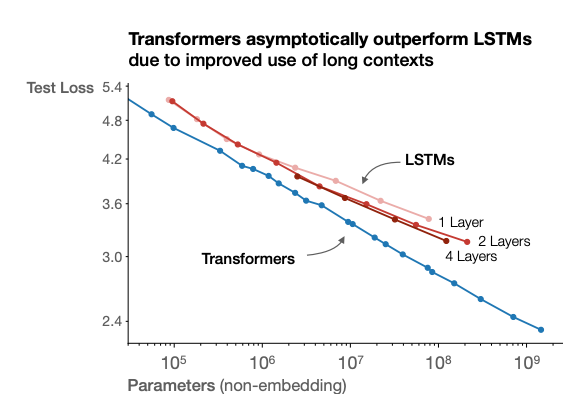
\includegraphics[scale=1]{linearScaling.png}
    \caption{Test loss (performance) against size (parameter count) of a model}
\end{figure}
\noindent SOTA for Transformers is currently Claude Opus, recently released by Anthropic. A few stats include Opus achieving 86.8\% on the MMLU (Undergraduate level multiple choice test) and 84.9\% on the HumanEval code benchmark \cite{opus}.
\\\\
Diffusion models gradually transform noise into a coherent image, based on learned data distributions. The SOTA is inherently more subjective in this area, but Midjourney version 5 is widely regarded as a front-runner in image generation. Midjourney can generate extremely detailed images from highly specific prompts.
\begin{figure}[H]
    \centering
    
\includegraphics[scale=0.4]{turtle.png}
    \caption{Generated using Midjourney with the prompt: `A scholarly turtle wearing glasses and a graduation cap, sitting in front of a stack of books. He has a wise and contemplative expression, as if lost in philosophical thought'}
\end{figure}
\noindent SOTA in video generation is clearly Sora, a recently released model from OpenAI which took the industry by surprise. Essentially working by diffusion but on multiple frames, Sora can also take in highly specific prompts and output detailed and realistic videos. 
\begin{figure}[H]
    \centering
    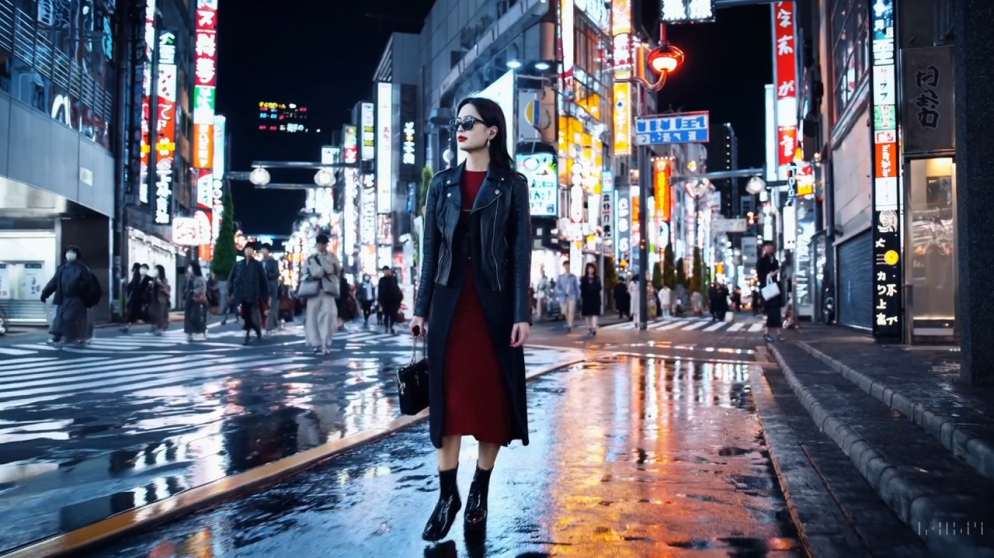
\includegraphics[scale=0.4]{sora.jpg}
    \caption{A frame from a Sora video, generated with the prompt: `A stylish woman walks down a Tokyo street filled with warm glowing neon and animated city signage. She wears a black leather jacket, a long red dress, and black boots, and carries a black purse. She wears sunglasses and red lipstick. She walks confidently and casually. The street is damp and reflective, creating a mirror effect of the colorful lights. Many pedestrians walk about.'}
\end{figure}
\subsection{Preserving Human Creativity}
The implication is that soon, we will be inundated with synthetic media and art. Whilst it is important to preserve human creations for philosophical reasons like maintaining the human identity, creative spirit and pride, there are two clearer motivators for building HumanMade:
\begin{enumerate}
    \item There will be free-market demand for authentic, human made creativity
    \item There is demand for GAI detection and tracking
\end{enumerate}
Expanding on the first - recent research (perhaps unsurprisingly) shows a clear bias in humans towards human made art \cite{anthropocentric}. In this study, participants in different groups were presented with the same piece of art, but labelled as either human made or AI made. These labels directly effected a participants' preference to buy the art, via biased perceptions of the creativity and awe they felt towards it.
\begin{figure}[H]
    \centering
    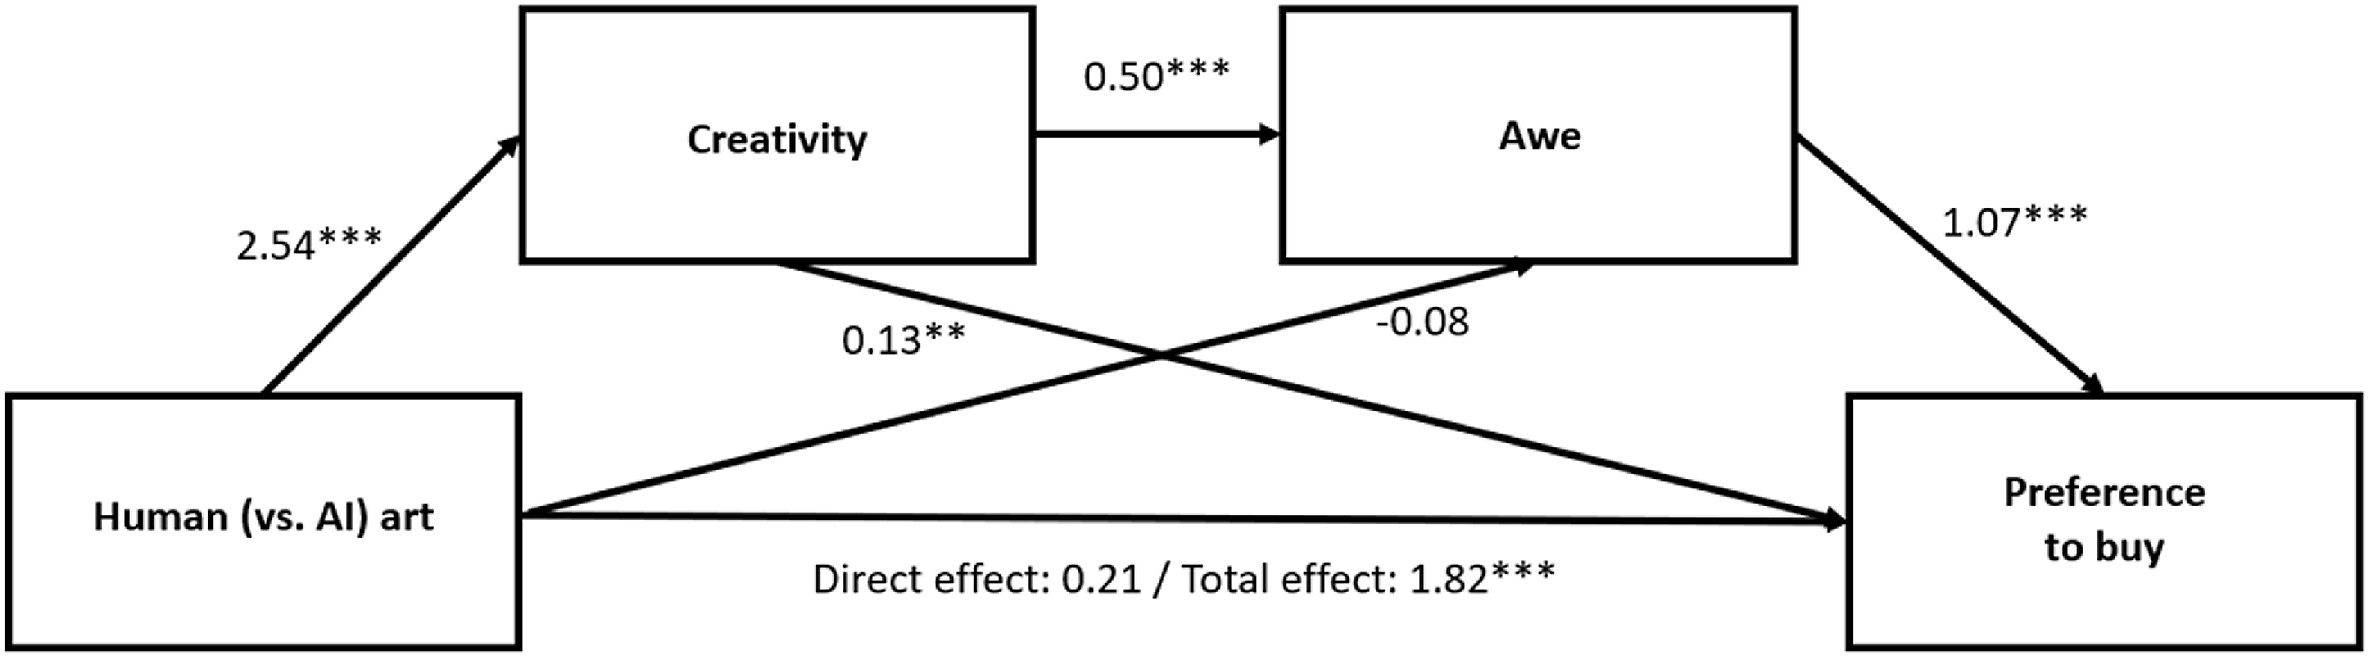
\includegraphics[scale=1]{biasDiagram.jpg}
    \caption{Indirect effect of human (vs. AI) art on preference to buy via perceived creativity and experienced awe.}
\end{figure}

\noindent On the second - tools which attempt to detect GAI are extremely popular (and for obvious reasons). For example GPTZero, a tool which attempts to detect AI generated text, has over 2.5 million users and partnerships with more than 100 organizations \cite{gptzero}. Industry-leading creative software developers Adobe have recently released Content Credentials, which is closer in spirit to what HumanMade is attempting. Both of these tools and more related systems will be further looked into subsequently.
\section{Background}
\subsection{Related systems}
We now look to analyse related systems and rate them out of 5 in three different categories - claimed capabilities, accuracy, and ease of use. This will give insight into what the best way to approach the development of HumanMade could be. In general, findings re-iterated the demand for a platform which does more than just attempt direct detection of AI. There were no holistic products with the aim of promoting human creativity.
\begin{table}[h]
    \centering
    \begin{tabular}{|M{3cm}|M{3cm}|M{3cm}|M{3cm}|}
    \hline
    System & Capabilities & Accuracy & Ease of Use \\ \hline 
    Adobe Content Credentials & 3 & 2 & 5\\
                           
\end{tabular}
\end{table}

\noindent Content credentials \cite{adobe} is advertised as, first and foremost, a way for creators to attach credit and usage details to their work, and second as a way to be transparent with AI generation. At the former it succeeds, however with the latter, content credentials only indicates the use of generation with regard to Adobe Firefly and other proprietary apps. This does not solve the issue of verifying any piece of AI generated content as specifically human made. Accuracy is poor as the system can easily be cheated - someone could screenshot a piece of digital work and then export it themselves. Ease of use is high as the feature is built right into industry leading apps used for content creation.

\begin{table}[h]
    \centering
    \begin{tabular}{|M{3cm}|M{3cm}|M{3cm}|M{3cm}|}
    GPTZero & 1 & 4 & 5\\
                           
\end{tabular}
\end{table}
\noindent GPTZero is a web interface that detects whether your pasted in text is AI generated or not. From testing by pasting in GPT-4 (the current state of the art for chatbots according to the widely used Huggingface arena leaderboard \cite{huggingface}) generated text, GPTZero performs fairly accurately, predicting 6/7 samples overwhelmingly correctly. GPTZero is a paid service beyond 7 free scans, and does not support any other types of content. Other systems tested perform at or worse than GPTZero.
\begin{table}[h]
    \centering
    \begin{tabular}{|M{3cm}|M{3cm}|M{3cm}|M{3cm}|}
    Sensity & 4 & 4 & 5\\
    \hline
\end{tabular}
\end{table}
\\\noindent Sensity is a leader in deepfake detection and has a high accuracy according to a recent study \cite{sensityStudy}. It has API, SDK and UI offerings.
\subsection{Issues with Direct Detection}
Despite accuracy scores for related systems initially looking positive, research shored up bigger picture concerns when considering a direct detection approach. GAI systems are improving at such a rapid pace that it will likely be impossible to keep up with them. 
\\\\Sensity mentions on their site, `As AI technology advances, new and more sophisticated techniques for generating realistic images emerge. Keeping up with these developments requires constant innovation and vigilance.' \cite{sensityBlog}. Sensity uses mainly ML techniques to identify GAI content \cite{sensityBlog}, and so of course the detection model is only as up-to-date as the data used to train it. When a cutting edge GAI model like Sora drops, content remains undetectable until detection techniques catch up again (assuming it is even possible for them to do so). \\\\Further, during the course of this third year project, Humbot was released \cite{humbot}. Humbot `humanizes' AI text to avoid detection by tools like GPTZero and Turnitin. Upon initial testing (\ref{fig:humbotFig}), Humbot works very well, and there are many examples and reviews of functionality on their site.  
\begin{figure}[h]
    \centering
    \begin{minipage}{0.45\textwidth}
        \centering
        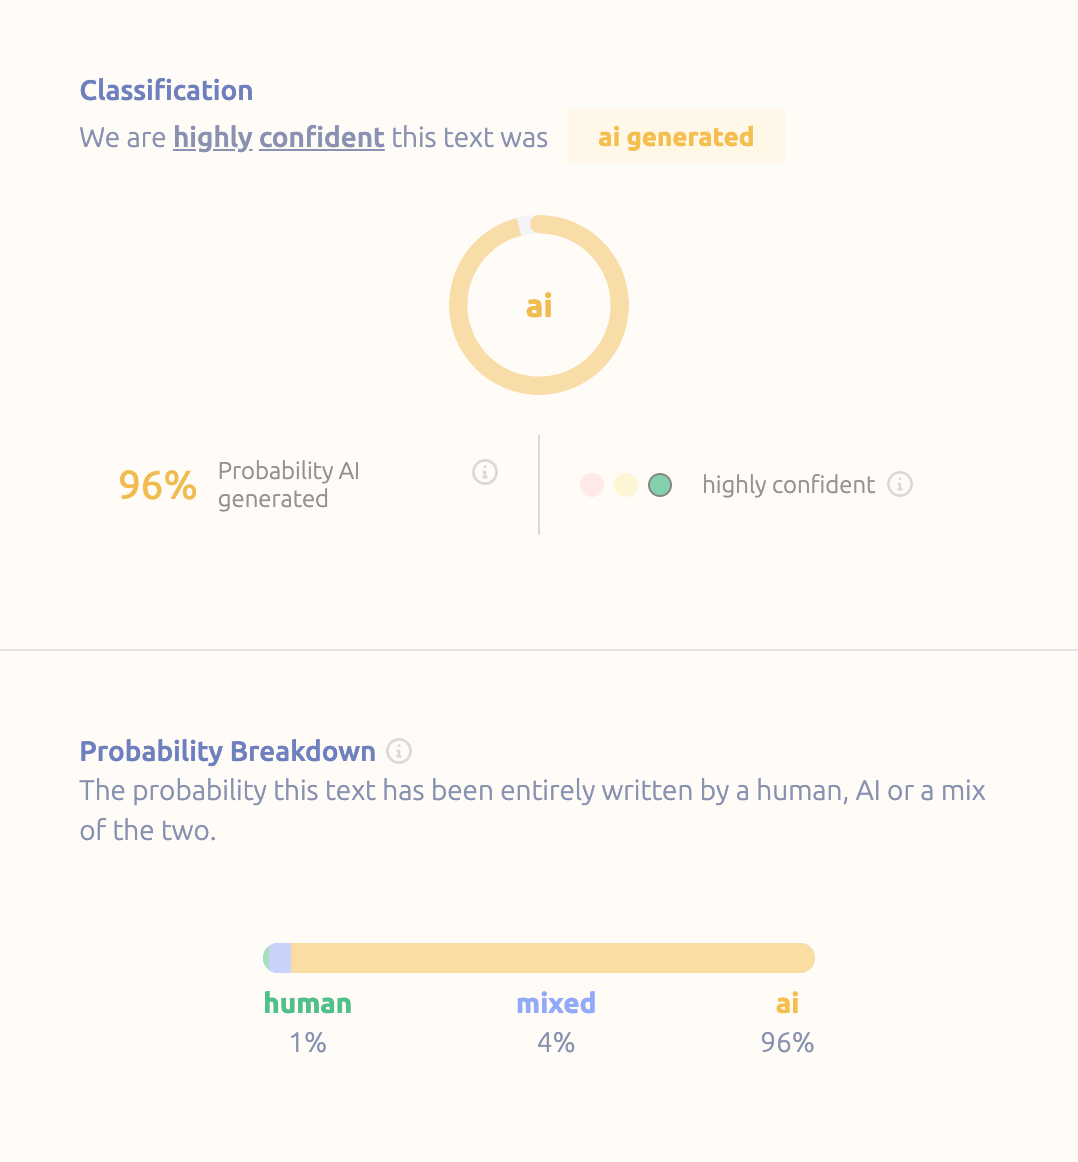
\includegraphics[width=\textwidth]{humbot2.png}
        \caption{GPTZero classification before using Humbot}
    \end{minipage}\hfill
    \begin{minipage}{0.45\textwidth}
        \centering
        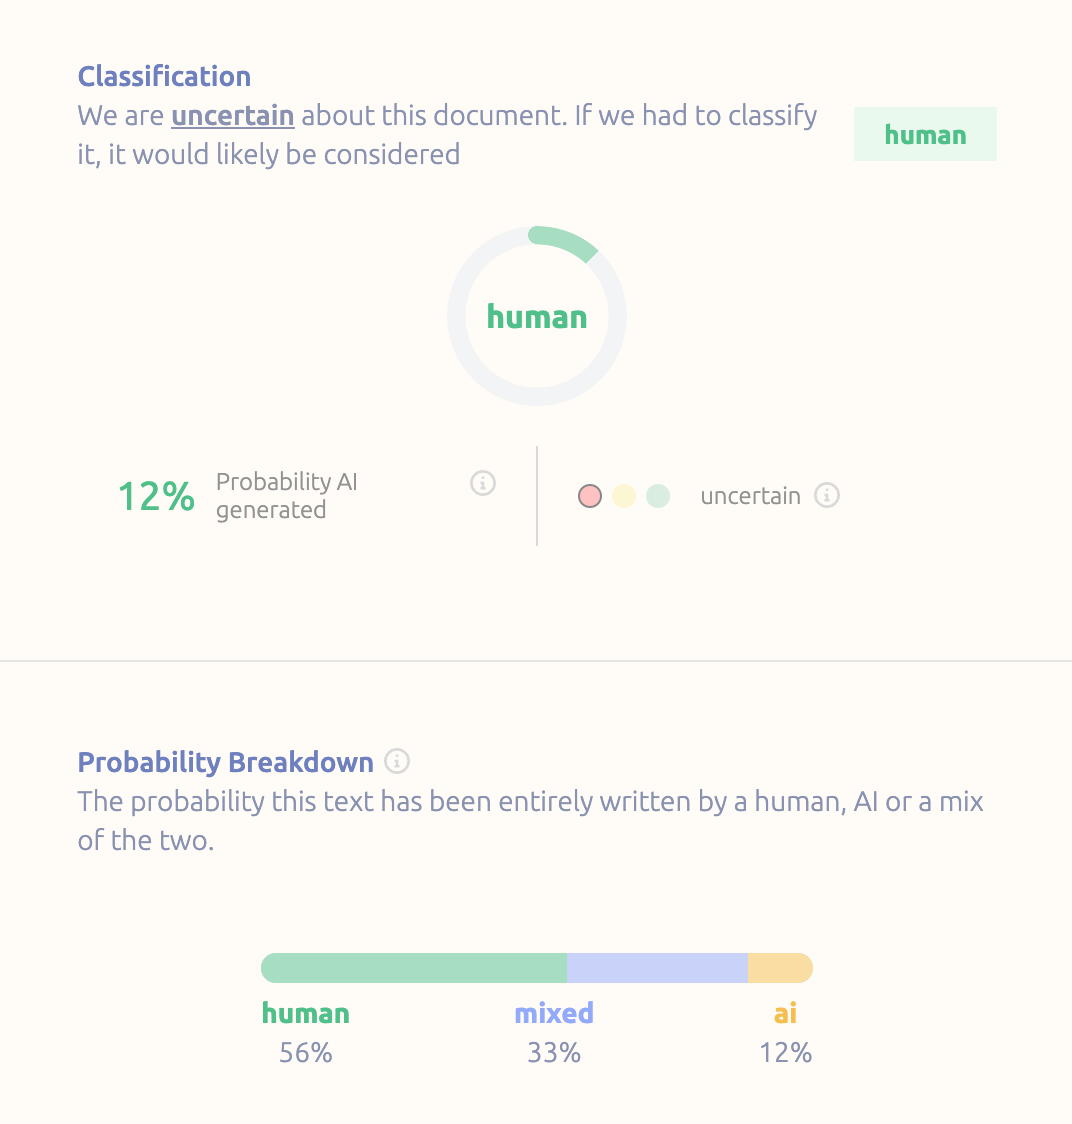
\includegraphics[width=\textwidth]{humbot1.png}
        \caption{Classification after using Humbot}
        \label{fig:humbotFig}
    \end{minipage}
\end{figure}

\section{Objectives}
After adequate research and analysis of the industry, the core objectives for HumanMade were then:
\begin{itemize}
    \item Creation of an intuitive and modern web app, allowing users to view and support human-made creations
    \item An easy way for creators to document their project and creative process to the app
    \item A way to ensure uploaded content is tamper-proof and traceable to a the author
\end{itemize}
TODO
\section{Design}
\subsection{Initial Design Ideas}
Initially, to circumvent the extensive issues with direct detection detailed previously, but to still allow for seamless and automatic verification, HumanMade was to work on an `evidence collection' basis. Evidence relating to the creative process itself would be collected, with the hope that this would give enough of a holistic input to whatever (likely ML) model was to be used to decide whether a creation was human or AI generated. Upon starting the project, there were some large caveats with this approach:
\subsubsection{Issues}
\begin{itemize}
    \item Data collection for training would be long \& an unproductive use of time. There were no existing datasets for my purpose.
    \item Data collected would be messy, with few consistent patterns. `Evidence' could have included screen recordings, screenshots, timelapses, etc. There would not have been many consistent underlying features or patterns to learn to make a fully automated ML approach work well.
    \item Not actually avoiding the fundamental issues stemming from direct detection. At some point, GAI technologies would probably get so good that they would be able to generate the evidence being used to identify human made creations. This leads to a further philosophical point detailed later, but it was clear a more holistic approach would be required. One that helps a consumer decide if a creation has had enough human investment to warrant supporting, and one that gives human creators a thriving community and the tooling to effectively share their work.
\end{itemize}
\subsection{Final Design}
The final design relies on some partially automated verification to give users an easier time identifying what might be human made, but the main approach revolves around the key concept of a progression timeline. 
\begin{itemize}
    \item Each progression timeline consists of `commits', akin to a git branch.
    \item Each creator-defined commit consists of files, a description, a percentage of completion, and an icon to denote whether AI was used.
    \item There is a simple interface to make any commit tamper-proof and traceable.
    \item There is a command line interface for easy publishing to the progress timeline for creatives.
\end{itemize}
\subsubsection{Advantages}
This approach had some inherent advantages, addressing the systemic issues we see with direct detection.
\begin{itemize}
    \item Generative AI has a very obvious `diffusion' progression. An image of pure noise is slowly transformed into the final output. This would be easy to spot on a progress timeline.
    \item The approach allows the community to decide the level of AI involvement in a creation they are comfortable with, as this is clearly a gray area. Certain AI tools which simply help a human creator be more effective in creating may not be inherently negative.
    \item The approach sidesteps the `arms race' between AI detectors and AI generators by allowing the community to decide for themselves what they think constitutes a human made creation. At a philosophical level, the best `neural network' one can use to achieve the aims of human made is the human brain.
    \begin{figure}[H]
        \centering
        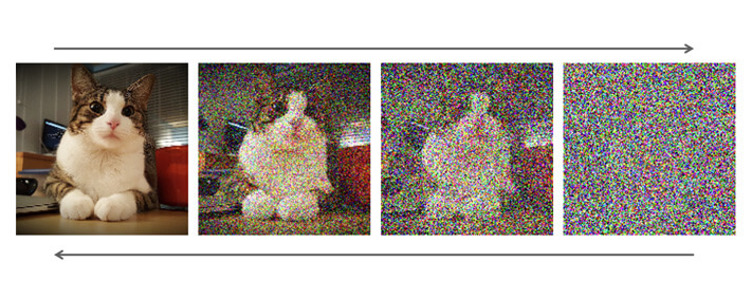
\includegraphics[scale=0.3]{catDiffusion.jpg}
        \caption{An example of the diffusion progression when generating a photo of a cat \cite{cat}.}
    \end{figure}
\end{itemize}
\section{Functionality}
There are then four main areas of development:
\begin{enumerate}
    \item \textbf{Web App} \\This involves giving users the ability to make new creations, commit to and view their progress timeline for each creation, and a marketplace for finished creations.
    \item \textbf{Machine Learning Microservice} \\This involves implementing the `partially automated verification' alluded to in the Final Design chapter. A metric for the continuity and progression across commits is computed using ML techniques.
    \item \textbf{Blockchain Interface} \\This involves creating a simple interface to make any commit tamper-proof and traceable by allowing users to record their commits to the blockchain.
    \item \textbf{Command Line Interface} \\This involves the creation of a command line tool that allows users to easily add commits to a progress timeline.
\end{enumerate}
We will look at the completed functionality of each before delving into implementation details.
\subsection{Web App}
\subsubsection{Homepage}
There is a basic homepage, currently only serving login functionality. This could easily be further extended to include account customization and creator profiles, but the main goal of the project was to build out the essential tools for the HumanMade proof of concept.
\subsubsection{Creations}
This is the tab of main importance in the application. Here a user can add new creations to their existing list, and within a creation is the `progress timeline'. 

Users commit to this progress timeline as they progress in their creation. A commit consists of:
\begin{itemize}
    \item a percentage indicating estimated completion
    \item files related to the creation
    \item a description
    \item an indicator as to whether AI was used
\end{itemize}
\textbf{Tagging:} A user can add tags to images in a commit. When the same tag is used across commits, the images are compared and a `similarity score' is computed. If the images do not correspond to a reasonable progression then this is marked on the progress timeline. This is a proof of concept for the partially automated verification alluded to in the Final Design chapter, allowing human creators to show and prove their progression more clearly to consumers.
\subsubsection{Marketplace}
This allows consumers to like and view finished creations, including the progress timeline, from any creator. Finished creations can currently only be filtered by most recent or most liked. Again, the marketplace is fairly basic in sacrifice of fleshing out the more experimental, non-obvious proof of concepts for HumanMade.
\subsection{Blockchain Interface}
When a user clicks on the link icon in the top right of any commit on the progress timeline, a MetaMask window will pop up. (If the user has not yet installed MetaMask, they will be prompted to do so). 
The user is prompted to login to their account, and the details of the transaction are displayed. If the user chooses to confirm the transaction, the file data in the commit and the user's ID will be hashed together and recorded on the blockchain via a smart contract function.  
\subsection{Command Line Interface}
The command line tool consists of 3 commands:
\begin{itemize}
    \item \textbf{login}, where the user specifies their email and later password in a hidden input
    \item \textbf{commit}, which takes arguments for the files, tags, description, percentage, and the creation ID to commit to
    \item \textbf{creations}, which lists all the creation ID's of the logged in user's creations.
\end{itemize}
The tool is written in Node.js and is run by using the \textbf{node} command, followed by the script path and required arguments. Example usage:
\begin{lstlisting}
node dist/humanmade.js login --email="sarifluca@gmail.com"
node dist/humanmade.js creations
node dist/humanmade.js commit --files="me.jpg" --inputTags="me" --description="A photo of me" --usedAI=false --percentage=50 --creationID=HGbyrdJjJSjwxXoKh9wO
\end{lstlisting}
\section{Implementation}
\subsection{Architecture}
\begin{figure}[H]
    \centering
    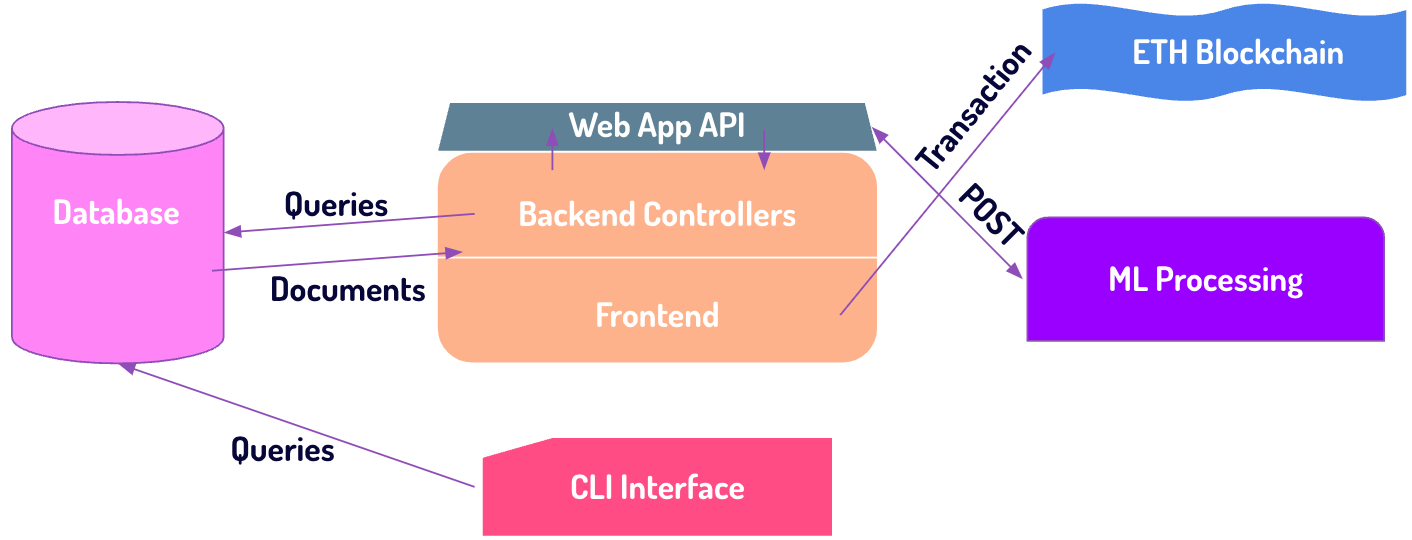
\includegraphics[scale=0.6]{architecture.png}
    \caption{System architecture for HumanMade. \cite{gpt4}}
\end{figure}
\subsection{Web App}

\subsubsection{Tech Stack}
After researching the many available web frameworks, middlewares and backend frameworks, I settled on a modern and scalable tech stack for the web app which would help me develop a reactive and robust app whilst writing clean code.
\begin{itemize}
    \item \textbf{SvelteKit} is a full-stack web framework which eliminates the need for a secondary middleware framework and allows for a simple and modern approach to building fast, reactive web apps. SvelteKit features server-side rendering, hydration, compilation minimisation, and plenty of other modern features to ensure an industry-level product. The framework enforces clean code and object-oriented programming practices. 
    \item \textbf{Tailwind} is an open source CSS framework. The UI is built by directly applying pre-defined styling classes to HTML elements. This allows for quick, consistent, and extensible styling, and works well with the component based methodology of SvelteKit. Tailwind has enamored developers for its customisability, configurability, and responsiveness.
    \item \textbf{Firebase} is a platform owned by Google offering a variety of tools and services to help developers build, improve and grow their apps. We will make use of the \textbf{Cloud Firestore} offering from Firebase as the primary database for the web app. Firestore is a NoSQL database that allows for fast querying, dynamic data storage and automatic scalability. Security and analytics are built into the product, and there is a generous free tier to facilitate testing and initial deployment of the project. Firestore also has an excellent modular web API that will play well with a JavaScript frontend. Additionally, Firebase offers \textbf{Cloud Storage}, a service for general blob storage of images, audio and video. This will be used for storing files associated with a commit. Again, security and scalability are integral. Finally, Firebase offers an authentication service which allows for the easy creation and maintenance of user accounts with industry-leading security standards.
\end{itemize}

\subsubsection{General Structure}
Roughly, a SvelteKit project consists of:
\begin{itemize}
    \item a \verb|src/| directory. This contains all the application source code.
    \item \verb|src/routes| contains all the application's pages and endpoints. SvelteKit uses a filesystem-based routing system, so the folder \verb|src/routes/marketplace| will contain the code for the page route \verb|/marketplace|
    \item In each route folder, eg. \verb|src/routes/marketplace|, there is a \verb|+page.svelte|, \verb|+layout.svelte|, and potentially a \verb|+page.ts| or \verb|+page.server.ts|.\\\\ \verb|+page.svelte| contains the HTML and any frontend JavaScript for the webpage. \verb|+layout.svelte| contains HTML that can be used to apply a general layout to any pages in the same or nested folders. \\\\\verb|+page.ts| and \verb|+page.server.ts| are like the `backend' for a page, and contain load functions (eg. to load data from a database) and form actions (functions which handle POST requests from a form element). There can also be a \verb|+layout.server.ts| which can contain a general load function which applies to any pages in the same or nested folders.
    \item \verb|src/lib| contains model code reused across the app. Components, utility functions, Svelte stores and type declarations all go here.
    \item \verb|src/routes/api| is where SvelteKit has you write any POST/GET API endpoints for your application. For example, adding a new folder named \verb|xyz|, containing a file named \verb|+server.ts| with a POST function, creates a new \verb|xyz| endpoint that handles POST requests.
\end{itemize}
\subsubsection{UI/UX}
\textbf{Components:} SvelteKit is a component based web framework. Components are custom UI elements you create out of standard HTML elements. This allows for consistent styling, functionality and reusability across the app. Each component consists of:
\begin{itemize}
    \item a \verb|script| section containing exported component prompts and any interactive functionality
    \item the HTML for the component
\end{itemize}
For example, this excerpt from a \verb|Button.svelte| component consists of click, size, submit and icon props. 
\begin{lstlisting}
<script lang="ts">
    export let click = () => {};
    export let size = 'md';
    export let submit = true;
    export let icon = ''
</script>
\end{lstlisting}
and these props are passed to an HTML \verb|<button>| element
\begin{lstlisting}
<button 
    on:click={click}
    type={submit ? 'submit' : 'button'}
    ...
\end{lstlisting}
These props can be given values when the component is actually used in a parent webpage.
\begin{lstlisting}
<Button size="md" icon="fa-brush">Create</Button>
\end{lstlisting}
\textbf{Styling:} As aforementioned, instead of styling directly with CSS, I used the more modern approach of going with a CSS framework, specifically Tailwind. Tailwind consists of many modular, pre-defined classes which let you style elements rapidly and inside the HTML. This div is styled to be a flexbox, with a specified width and rounded corners.
\begin{lstlisting}
<div class="flex flex-col gap-2 w-6/12 rounded-2xl bg-opacity-80 bg-primary p-5">
\end{lstlisting}
For example, the \verb|flex| class is defined by Tailwind as:
\begin{lstlisting}
.flex {
    display: flex;
}
\end{lstlisting}
Notice the background is set to be \verb|bg-primary|. Thanks to Tailwind's configurability, we can specify a color palette, font family and font sizes in a \verb|tailwind.config.js|, and Tailwind will automatically incorporate our choices into the generated CSS class options.
\begin{lstlisting}
colors:{
    'primary': '#2E4052',
    'secondary': '#FFC857',
    'tertiary': '#BDD9BF',
    'quaternary': '#412234'
},
\end{lstlisting}
\textbf{Icons:} Iconography is important for aesthetics and accessibility. Font Awesome is a library that provides high-quality minimalist SVG icons for websites. It exposes these assets via CSS classes, meaning just as with Tailwind we can reference icons directly in the markup of our website, providing consistency and cleanliness across the codebase. 
\subsubsection{Authentication}
Firebase has simple API methods for creating and authenticating users with an email and password combination. The authentication flow is as follows:
\begin{enumerate}
    \item In the event that either method is successful, a result object is returned with a user property containing the user ID, display name and email.
    \item We extract and save these into a custom User type object, (and write a user document to the Firestore database if this is a new user), and then set a `user' cookie value to this object (serialised).
    \item We then have a \verb|+layout.server.ts| at the root of \verb|src/routes| containing a load function which returns the user object from the cookie.
    \item  This load function applies to all webpages, safely and efficiently exposing the user object to all pages which require it.
\end{enumerate}
Using Firebase authentication with Firestore makes the app seamlessly secure. We can write custom security rules in Firestore to restrict user access to certain documents in the database. For example, here we ensure that a creation can only be edited by the original owner of the creation:
\begin{lstlisting}
match /creations/{document=**} {
  allow write: if request.auth.uid == resource.data.uid;
}
\end{lstlisting}
Firebase authentication handles attaching an auth token to any database requests the user makes, giving Firestore access to the \verb|request.auth| object to use in security rules.
\subsubsection{Reactivity \& Updates}
To ensure a reactive and responsive experience for users, we develop a way to keep the client and server in sync with a clean and elegant approach.
We take advantage of Svelte reactive stores and Firestore realtime listeners.\\\\
\textbf{Svelte Stores:} These are helpful for managing global state across components. The type of store we use is \verb|writable|, where we store arrays either of type \verb|Creation| or \verb|Product|, for the creation and marketplace tabs respectively. We can read and write values to these arrays, via the \verb|update| and \verb|set| methods of the store, and more importantly we can now subscribe to the store. Then, any components relying on the store values are automatically re-rendered by SvelteKit upon updates to the store. For example, this \verb|each| loop will re-render any of the necessary \verb|CreationDiv| components upon any updates to the \verb|creations| store.
\begin{lstlisting}
{#each $creations as creation (creation.id)}
    <CreationDiv {creation}></CreationDiv>
{/each}
\end{lstlisting}
\textbf{Realtime Listeners:} These simply subscribe to a collection of documents in the Firestore database, triggering upon any changes to the collection. Firebase returns a collection of \verb|DocumentChange|s, which supplies the document which was updated and the type of update (added, modified or removed).
\\\\
Using these two concepts, we can map changes we see from the listener to changes in the store, allowing us to efficiently update UI every time the database state changes. To do this mapping cleanly, we implement a \verb|Listener| wrapper class for each store, which gives us methods to easily update the store from listener document updates. 
\begin{lstlisting}
abstract class Listener<T>{
    abstract update(struct: T): void;
    abstract remove(struct: T): void;
    abstract add(struct: T): void;
    abstract docToType(doc: DocumentSnapshot): T;
}
\end{lstlisting}
\noindent
The diagram below illustrates the approach at a high level.
\begin{figure}[H]
    \centering
    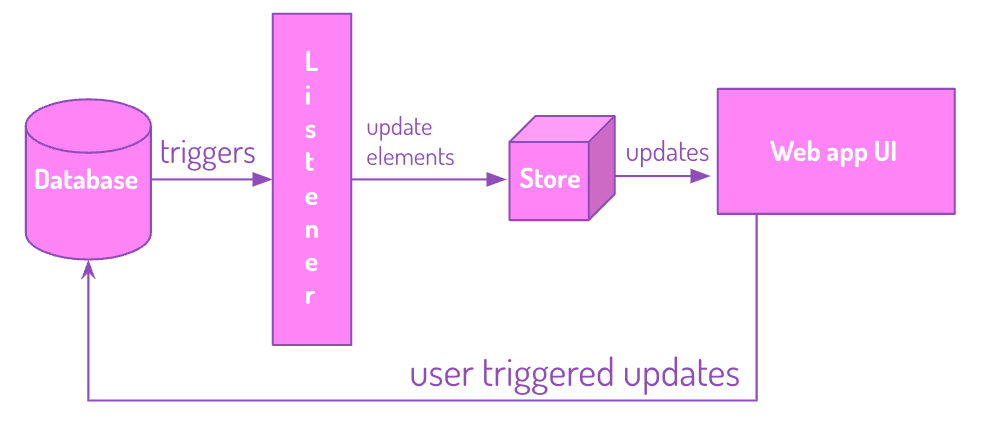
\includegraphics[scale=0.8]{reactivity.png}
    \caption{Reactivity system for HumanMade\cite{gpt4}}
\end{figure}
\subsection{Machine Learning Microservice}
\subsubsection{Tech Stack}
\begin{enumerate}
    \item \textbf{TensorFlow} is a free and open-source machine learning library from Google, providing state of the art models and APIs in Python.
    \item \textbf{Flask} is a micro web framework written in Python, perfect for setting up a simple API for the microservice with which the main web app can interoperate. 
\end{enumerate}
This microservice handles computation of the similarity score between images of the same tag across commits, as described in the functionality section.
\subsubsection{Firebase Storage} Any images uploaded in a commit are stored in cloud storage, with a \verb|+| separated filename consisting of the image \verb|tag|, \verb|file.type| and the current date to avoid the chance of duplicate filenames.
\subsubsection{Data Flow} The data flow when interacting with the ML processing microservice is as follows, and is also detailed in the below diagram.
\begin{figure}[H]
    \centering
    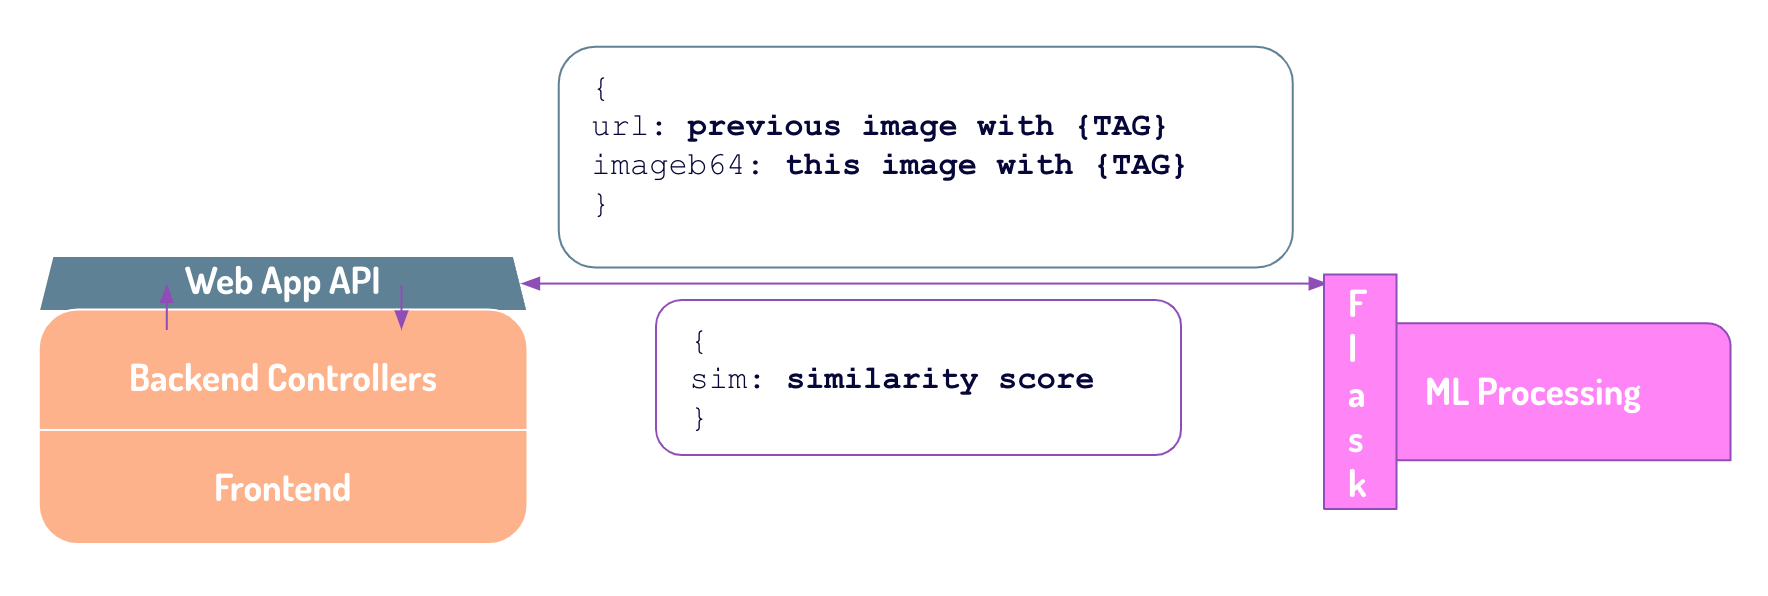
\includegraphics[scale=0.6]{ml.png}
    \caption{Data flow diagram for the ML microservice}
\end{figure}
Upon a new commit to the progress timeline containing an image tagged \verb|{tag}|, and given there is an image with tag \verb|{tag}| in the previous commit:
\begin{enumerate}
    \item The base 64 encoding of the image in the current commit, and the URL of the image in the previous commit are posted in JSON to the \verb|imageSimilarity| API endpoint. 
    \item The microservice processes the images (detailed in the next section), and return back a similarity score to the web app API's request.
    \item The endpoint returns the similarity score to the frontend, and this is displayed on the progress timeline if below a certain threshold.
\end{enumerate}
\subsubsection{Similarity Computation} ResNet50, a 50 layer Convolutional Neural Network provided by the Tensorflow library, is used to extract a high level feature vector from each of the images. These two vectors are then compared using cosine similarity.\\

Firstly, we preprocess the images:
\begin{itemize}
    \item Images are received by Flask in a POST method. The images are downloaded (as required) and written to \verb|.jpg| files. 
    \item Images are size adjusted (ResNet required images to be in \verb|224x224| resolution) and converted to a 3D array (width by height by color channels, (224,224,3)). ResNet actually takes input in 4D, where the first dimension represents batch size, so we need to expand our array to dimensions (1,224,224,3).
    \item Finally the TensorFlow provided \verb|preprocess_input()| function scales and normalises pixel values of the image.
\end{itemize}
Then, we can extract a feature vector for each image: ResNet50 is a classification model, with its final layer consisting of 1,000 different classes. We do not want to classify our images - so, we stop the model at an intermediate layer, giving us a high level feature vector describing the images. We can do this with the provided \verb|Model| python class, which lets us specify a base model and the output layer. ResNet50 consists of pooling, convolutional and ReLU activation layers. 

We choose a late convolutional layer to stop at. These layers are where kernels/filters are applied to the image to better detect high level abstract features \cite{convNN}, which is what we want when comparing similarity. The general shape, color and vibe of an image should not change drastically commit to commit as a user is working on a project, whereas specific pixel values and details could and should be allowed to.
\begin{figure}[H]
    \centering
    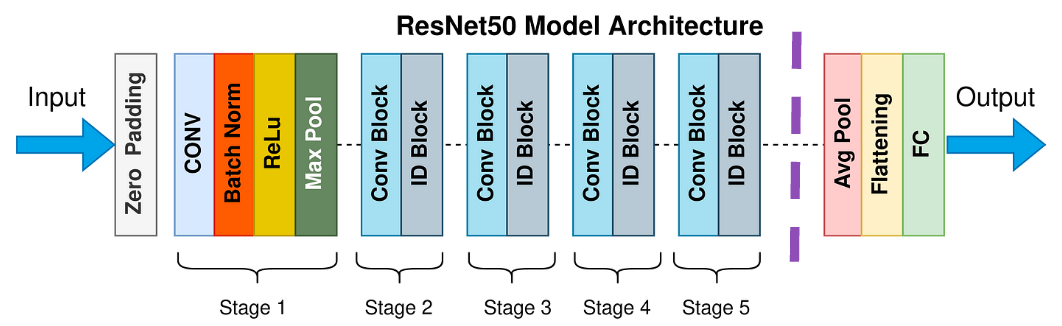
\includegraphics[scale=0.8]{resnet.png}
    \caption{We look to cut off ResNet's output early.}
\end{figure}
Finally, we used cosine similarity (\verb|1-cosine(vec1, vec2)|) to compare the feature vectors. At a high level we can think of this as measuring the `direction' of the vectors in \verb|n|-dimensional space and seeing how closely they align.

\subsection{Blockchain Interface}
\subsubsection{Tech Stack}
\begin{itemize}
    \item \textbf{MetaMask} is a leading self-custodial cryptocurrency wallet, used to interact with the Ethereum blockchain. Users can access their wallet and perform transactions with ease, and without having to send their private key across a network. The MetaMask Chrome extension provides a modern way for web apps to integrate with the blockchain.
    \item \textbf{Solidity} is the defacto programming language for implementing smart contracts, mainly on the Ethereum blockchain. A smart contract can be thought of as a self-executing contract that a user can interact with by sending crypto to.
    \item \textbf{Remix} is an open-source IDE widely used for smart contract development. We use Remix to compile, deploy and test our smart contract. 
    \item \textbf{Web3.js} is a collection of open-source libraries that primarily provides an abstracted interface for communication with an Ethereum node, as well as other helpful utility functions. This is the layer we use to interface with the Blockchain from our frontend JavaScript.
\end{itemize}
\subsubsection{Smart Contract Development}
The code for the smart contract is fairly short, consisting of a 
\\\verb|makeCommit(string[] fileHashes)| function, which emits an event\\ \verb|CommitMade(msg.sender, hash)| that could be used to trigger actions in other decentralized applications in the future. For the purpose of this application, the \verb|makeCommit| function is of importance, as this is what gets recorded in a transaction on the blockchain when invoked.\\\\
We then use Remix to compile and deploy the contract. The Solidity contract is compiled down to bytecode, and can then be deployed to either:
\begin{enumerate}
    \item the Ethereum mainnet
    \item a Ethereum testnet
    \item a virtual JavaScript network in the browser
\end{enumerate}
We opt for option 2,  deploying the contract to the Sepolia testnet, a proof-of-stake network designed to mimic the operating environment of the mainnet but existing on a separate blockchain ledger. We can receive free ETH to use on this testnet via many of the available Sepolia `faucets'.

This is in fact the only viable option. At least until it is required in production, we don't want to have to pay the (sometimes exorbitant) gas fees required to commit a contract (or conclude any transaction) to the mainnet during testing, which option 1 would require. We also want to be able to test our contract using an actual transactions signed with MetaMask, which would not be possible if we deployed our contract to a virtual browser network with option 3.

Deploying via Remix to the Sepolia testnet, (paying gas fees using a wallet with Sepolia ETH in it), gives us the contract address and contract Application Binary Interface (ABI), which is all the information we need to make a transaction with the contract. The ABI simply represents the contract in a structured format, so that calls to the contract can be encoded into bytecode which the Ethereum Virtual Machine can process.
\begin{figure}[H]
    \centering
    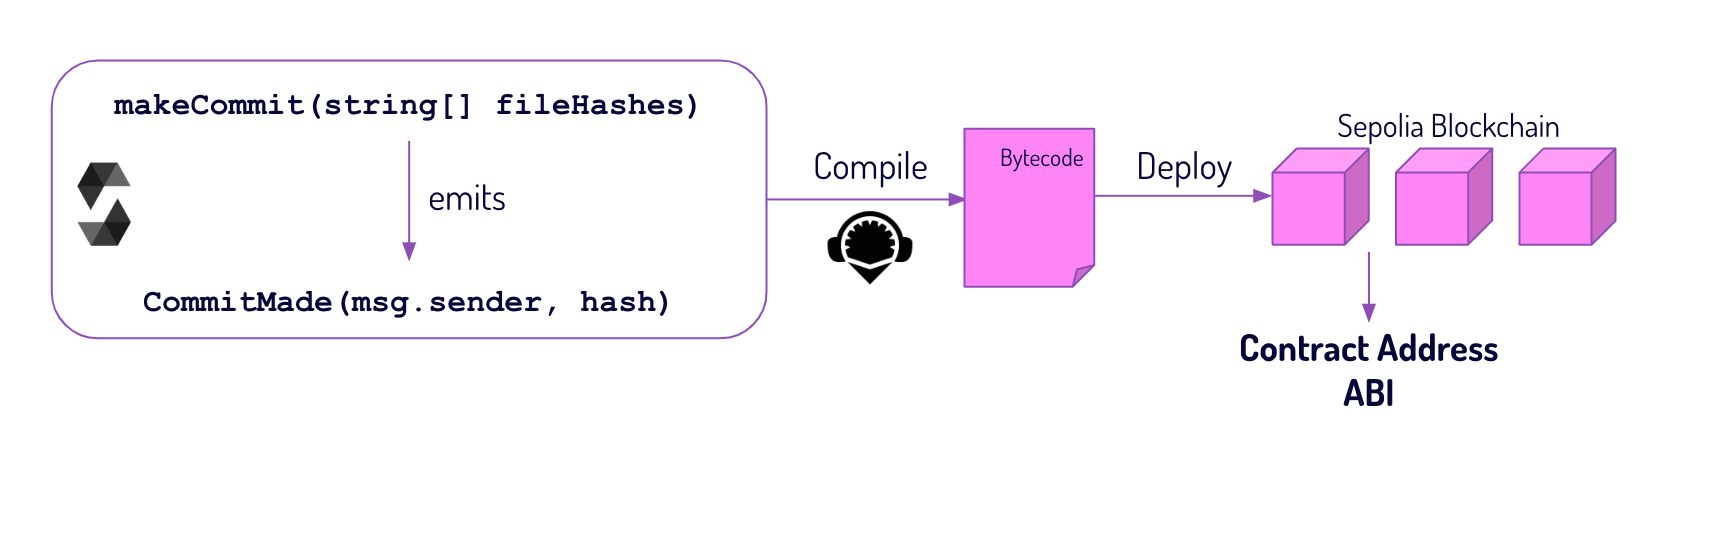
\includegraphics[scale=0.6]{deploy.png}
    \caption{The process for compiling and deploying the Solidity smart contract}
\end{figure}
\subsubsection{Communication Setup}
To communicate with the blockchain using the Web3.js interface, we need to pass the \verb|Web3| constructor a `provider'.
A provider is an object which communicates with an Ethereum node, supplying essential properties and methods which adhere to the Ethereum Provider API standard. MetaMask supplies us with this object when installed, injecting a \verb|window.ethereum| object into the browser for web apps to make use of.
\begin{lstlisting}
const web3 = new Web3(window.ethereum);
\end{lstlisting}
Now that \verb|Web3| is invoked with a valid provider, we can create a Contract object which will let us execute our contract methods on the chain. This is where we need the contract address and ABI:
\begin{lstlisting}
const contract = 
    new web3.eth.Contract(JSON.parse(abi), address);
\end{lstlisting}
Now, we have access to all the methods we need to perform a transaction on the chain.
\subsubsection{Performing Transactions}
We want the transaction we perform to contain content related to the files in the progress timeline commit, and to the user themselves. So, hash each file in the commit with the user ID, and pass it to our contract method. This way, each commit is tamper-proof and traceable, with the original content and creator recorded permanently on the blockchain ledger.
\begin{figure}[H]
    \centering
    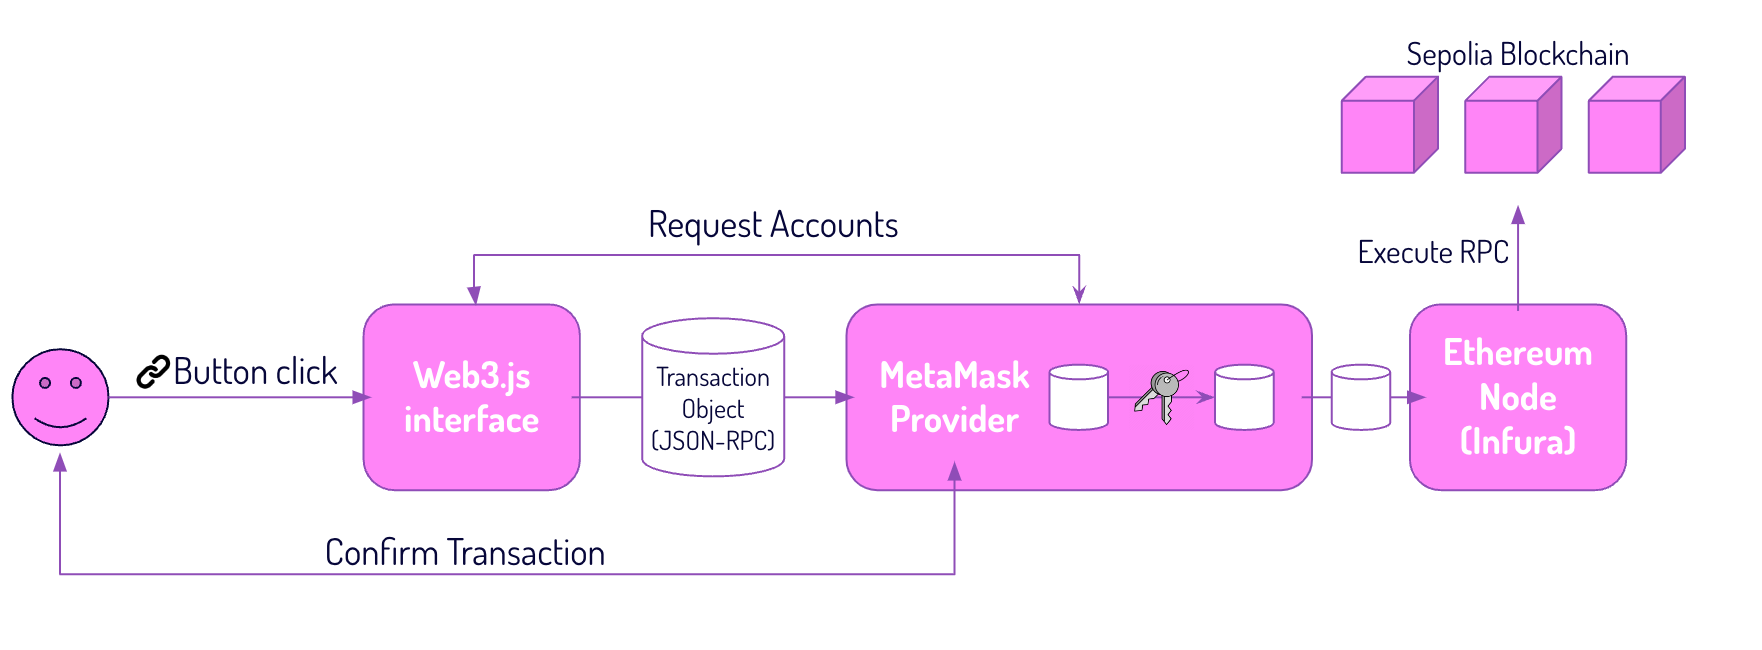
\includegraphics[scale=0.6]{bchain.png}
    \caption{The full process of performing a transaction end-to-end}
\end{figure}
Upon a user clicking the `link' icon on a progress timeline commit:
\begin{enumerate}
    \item We get the contract address and ABI. These are stored on the server for safety, so the backend controller makes a call to a \verb|blockchainCommit| API endpoint to get these details first. 
    \item We request access to the MetaMask accounts, obtaining the user's wallet address.
    \item We create the transaction object - a simple JavaScript object where we pass:
    \begin{itemize}
        \item the receiver, in this case the contract address
        \item the sender, in this case the user's wallet
        \item a data string the Ethereum Virtual Machine can interpret as a command, in this case a string of bytecode representing a call to the contract method \verb|makeCommit|. We can obtain this using the Contract object we created earlier in the setup phase.
        \begin{lstlisting}
data: contract.methods.makeCommit(commit.hashes).encodeABI()
        \end{lstlisting}
        \item the user's transaction count (the nonce, which provides a unique ID for each transaction and ensures transactions are ordered and executed correctly)
        \item gas fees and the gas limit. We calculate the fee based on the latest blocks gas fee, and the limit based on the size of the transaction object.
    \end{itemize}
\end{enumerate}
Finally, we perform the transaction, 
\begin{lstlisting}
const txHash = await web3.eth.sendTransaction(txObject);
\end{lstlisting}
and save the hash to the database, signifying that the commit has been recorded on the blockchain.
\subsection{Command Line Interface}
\subsubsection{Tools Used}
\begin{itemize}
    \item \textbf{Node.js} is the defacto language and runtime for out-of-browser JavaScript. It allows us to write our command line tool in Typescript, make network requests and take advantage of the flourishing library ecosystem.
    \item \textbf{Yargs} is a popular library for building command line tools in Node.js, providing an easy and abstracted way to specify commands and their functionality.
    \item \textbf{Inquirer} is a popular library for building command line interface prompts.
\end{itemize}
\subsubsection{Authentication}
The user needs to be able to authenticate directly with Firebase through the command line interface, in order to securely commit to a creation.
\begin{itemize}
    \item The user will specify their email when using the login command.
    \item Once executed, the command will prompt the user for their password, using Inquirer to ensure the input is hidden.
    \item We can then use the same Firebase authentication methods provided for node as we did in the web app, giving us a \verb|result| object in return.
    \item The difference now is we need to manually handle storing the authentication token for the user. We can extract the JSON Web Token (JWT) used to identify the user to a Firebase service from the \verb|result| object, and cache this in a text file. 
    \begin{lstlisting}
let token = await res.user.getIdToken();
await fs.promises.writeFile("./HumanMade/token.txt", token);
    \end{lstlisting}
    The user can then use the command line tool freely until the token expires, in which case they would use the \verb|login| command again. 
\end{itemize}
The Firebase SDK which would normally sign the requests for a user automatically, as in the web app, only works within a browser environment. We must instead use the Firebase REST API in conjunction with the JWT.
\subsubsection{Firebase REST API}
We use the fetch API to interact with Firebase via the REST API. The base URL for all requests we will make is of the following form:
\begin{lstlisting}
const baseUrl = https://firestore.googleapis.com/v1/projects/${projectId}/databases/(default)/documents
\end{lstlisting}
In every (POST) request to the API, we send the JWT along in the \verb|Authorization| property of the header. This lets Firebase Firestore identify the user querying the database, ensuring database requests adhere to security rules.
\\\\
If we want to query data, as in the case of querying creation IDs with the \textbf{creations} command, we can post a \verb|StructuredQuery| JSON object to the \verb|`${baseUrl}:runQuery`| endpoint. A \verb|StructuredQuery| object can specify all the attributes we would normally use when querying using the Firebase SDK, including \verb|where| clauses and a \verb|from| property to specify which collection we would like to query from. 
\\\\
Creating data, as in the case of creating a new commit with the \textbf{commit} command, we similarly POST a JSON object specifying the fields of the document we want to create, along with the JWT in the header. In the process of creating a commit we also handle image similarity across any images with the same tag, querying the \verb|/imageSimilarity| microservice endpoint.
\section{Testing}
postman, lighthouse
\section{Conclusions}
\subsection{Limitations}
Limitations of the project are mainly due to restrictions on time. Much of the choice of what to work on was dictated by how obvious and easy the work would be. Functionality which was non-trivial and added to the proof-of-concept for HumanMade was prioritised, and areas which could obviously be fleshed out with little need for creativity were understated.
\begin{enumerate}
    \item The marketplace has limited functionality. It is hard to find creations a user may be personally interested in, there is no fuzzy search, a lack of creator profiles and a following system, and no in-built buy or sell functionality. This would take time but be fairly simple to implement with modern technologies and libraries, and would flesh the project out to a fully usable one-stop platform for human creativity.
    \item Currently, we only transact on a blockchain test-net instead of an actual production chain. Test-nets still implement the same cryptographic techniques that make blockchain a secure technology, providing a tamper-proof ledger with which we can record commits on. However, network security may not be as robust; the security of a chain is dependent on the number of nodes participating in the network, and there are fewer of these on test-nets due to their being less financial incentive (the tokens on these test-nets have no real world value). Further, support for a test-net like Sepolia could very well be discontinued.\\\\We did successfully implement a version of the blockchain interface which commits directly to the Ethereum Blockchain with minimal effort, since the transaction process for Sepolia is much the same, however this brings about separate limitations in the form of the high gas fees required for a transaction that (especially at busy times) can be non-negligible.
    \item Extra effort is still required on the part of the creator to use the application, but lots of thought was put into reducing this workload, resulting in the command line utility.
    \item Creative endeavours are rarely so linear in their progression. Perhaps adding support to branch/merge as in git would help creators express their progression more seamlessly to consumers.
    \item There was a lack of market research undertaken to gauge what features real-life creatives would value. This was due to a lack of interaction and tight deadlines.
\end{enumerate}
\subsection{Future Development}
As aforementioned, a lot of future development consists of fleshing out obvious areas of the application which were neglected due to tight deadlines.
\begin{enumerate}
    \item Additional ML techniques for the automatic verification of auditory and written media (the two other types of creation other than visual) could be added. Also, further research could uncover better techniques to gauge the credibility of a human progression across the timeline.
    \item We could transact on a blockchain main-net with no gas prices - blockchains such as Nano \cite{nano} exist but were only discovered after completion of the project, and have much poorer developer ecosystems. 
    \item The command line utility can be fleshed out further into a full git-like tool, providing branching, merging, deletion and restructuring capabilities of the timeline.
    \item Adding recommendations (could involve using collaborative filtering ML methods), further filtering options, fuzzy search and creator profiles to the marketplace would help artists find their audience more easily, and help consumers find the art they want to support.  
    \item The concept of a upvote/downvote system was floated early in the project - where creations with more upvotes (potentially a sign of legitimacy) are promoted and shown to more users. Community driven recommendations have been shown to work well across a multitude of social media platforms already.
\end{enumerate}
\subsection{Contributions}
\begin{enumerate}
    \item This is the first platform of its kind for human made creations. Whether the platform itself gains popularity, it is a useful blueprint and inspiration for what will inevitably become a highly in-demand service.
    \item We address some of the large issues with popular AI detection tools, bringing a holistic viewpoint to the conversation of generative AI detection. It is important to avoid the speciesist trap that generative AI will always be detectable against human creations, as pointed out in the Motivations chapter.
    \item We use an innovative combination of approaches and choices driven by research of the current state of the art and future projections of the technology. This includes tamper-proofing and tracing with blockchain, and progression detection with Convolutional Neural Networks.
    \item We make use of scalable, modern and future-proofed tooling, using a young and popular reactive compiler-based framework in SvelteKit and a fast, secure database in Firebase.
\end{enumerate}
\section{Project Management}
\subsection{Methodology}
HumanMade involves a lot of integration and experimenting with cutting-edge technologies that I didn't necessarily have previous experience with, so it was important to keep the development process flexible as well as consistent.

Agile lent much needed adaptability and flexibility to the process. Changes in scope were inevitable due to a foray into a completely new type of platform, incorporating modern technologies. We worked on weekly sprints based off of a GANTT chart (specified in the specification document) which provided us with a high level timeline and milestones to hit for the project. For a sprint, we would set a specific objective to complete a certain component or piece of functionality by the end of the week. Then, we could reassess the GANTT chart and formulate the next sprint, ensuring we stayed on track to deliver a finished product by the end. Agile further helped in this regard by ensuring we broke up work into manageable modules, which could be continuously delivered and integrated into the project. This avoided scenarios where a certain component could be worked on for a substantial period of the project only to not work or integrate correctly. For example, setting up a basic image similarity endpoint with a Flask app was one sprint, and in a separate sprint we delved deeper into using a machine learning approach.
\begin{figure}
    \centering
    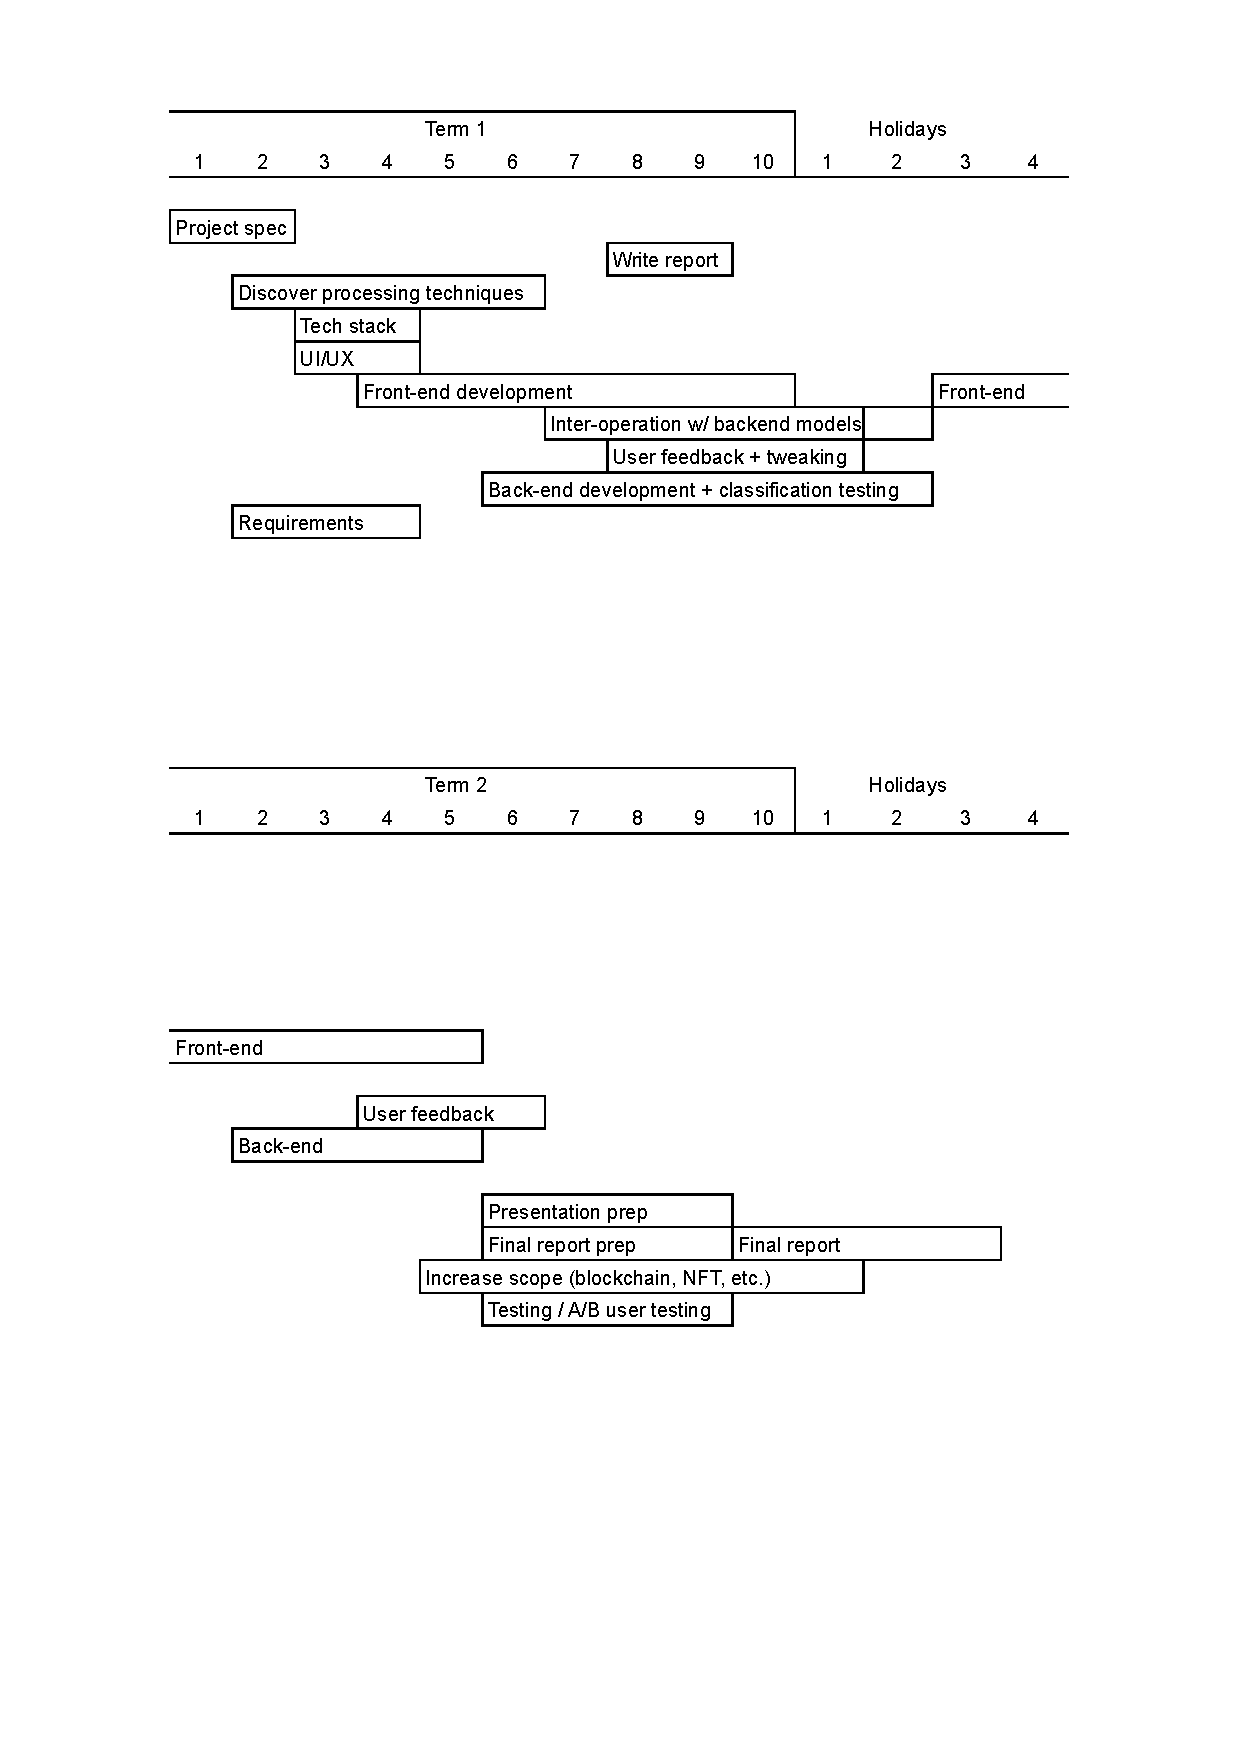
\includegraphics[scale=0.5]{gantt.pdf}
    \caption{The GANTT chart used throughout the project}
\end{figure}
\subsection{Tools}
To aid with the above methodology:
\begin{itemize}
    \item Trello was used for bug tracking and defining sprints and tasks to complete
    \item GitHub was used for version control, allowing development of experimental breaking features on separate branches, and providing an up-to-date backup for work by making it easy to consistently commit progress.
    \item Visual Studio Code was used for development. This integrated environment has syntax and completion support for many of the technologies that were being used including Svelte, Python, and TypeScript.
\end{itemize}
\subsection{Risk}
Risks were laid out at the start of the project, and relevant steps were taken to mitigate them:
\begin{itemize}
    \item Hardware failure, mitigated by:
    \begin{itemize}
        \item Keeping regular backups
        \item Using git consistently
    \end{itemize}
    \item Lack of expertise in the areas of development, mitigated by:
    \begin{itemize}
        \item Scheduling regular check-ins with supervisor
        \item Taking advantage of online material and LLM's like ChatGPT
    \end{itemize}
    \item Cloud services being used (GitHub) become unavailable, mitigated by:
    \begin{itemize}
        \item Keeping regular backups of report and code files on a third party like Google Drive
    \end{itemize}
\end{itemize}
\subsection{Progress against Original Objectives}

\section{Philosophy of it}
\newpage
\bibliography{finalReport}

\end{document}